\chapter{Firewall}
Un \textbf{firewall} è un apparato software o hardware configurato per ammettere, abbattere o veicolare (proxy firewall) connessioni tra due aree di rete con differente \textit{livello di fiducia}. Ad esempio, un firewall perimetrale viene normalmente posto su un gateway per separare la rete locale (alto livello di fiducia) da internet (livello di fiducia minimo). Lo scopo finale del firewall è quello di offrire un'interfaccia configurabile tra due segmenti di rete con diversi livelli di fiducia. L'interfaccia deve essere configurabile attraverso security policy basate su due principi: \textit{least privilege} (l'utente deve avere solo i privilegi essenziali al proprio lavoro) e \textit{separation of duties} (separazione delle funzioni). Esistono due politiche per l'applicazione delle regole:
\begin{enumerate}
	\item \textbf{Policy default-deny}. Viene permesso solo ciò che viene dichiarato esplicitamente, il resto viene vietato;
	\item \textbf{Policy default-allow}. Viene vietato solo ciò che viene dichiarato esplicitamente, il resto viene permesso.
\end{enumerate}
Tutti i firewall utilizzano la politica default-deny, poiché garantisce una maggiore sicurezza e una maggiore accuratezza nella definizione delle regole rispetto alla politica default-allow, anche se quest'ultima consente una configurazione più semplice. La configurazione di un firewall richiede profonda conoscenza dei protocolli di rete e di network security: un errore nella configurazione può rendere inutile il suo utilizzo.

L'analisi dei pacchetti che costituiscono il traffico, secondo i criteri di sicurezza formalizzati dalle regole, si traduce in una delle seguenti azioni:
\begin{itemize}
	\item \textbf{Allow}. Il firewall lascia passare il pacchetto;
	\item \textbf{Deny}. Il firewall blocca il pacchetto e lo rimanda al mittente;
	\item \textbf{Drop}. Il firewall blocca il pacchetto e lo scarta senza inviare alcuna segnalazione al mittente.
\end{itemize}
Solitamente i firewall non prevedono il blocco del pacchetto e il rinvio dello stesso al mittente per evitare uno spreco di banda. È del tutto sbagliato pensare che tutti gli attacchi provengano da Internet (o altra rete al di là del firewall): tanti attacchi possono benissimo provenire dalla rete LAN da proteggere; per questo motivo un firewall non deve solo controllare i pacchetti in entrata, ma anche quelli in uscita.

Nel corso degli anni i firewall si sono sviluppati, dando luogo a diverse tipologie:
\begin{itemize}
	\item \textbf{Packet filter}. Un packet filter firewall o \textit{stateless} firewall analizza ogni pacchetto che lo attraversa singolarmente, senza tenere conto dei pacchetti che lo hanno preceduto. In altre parole, la decisione presa all'istante $t$ non è condizionata dalle scelte fatte per i pacchetti precedenti. In tale analisi vengono considerate solo alcune informazioni contenute nell'header del pacchetto: indirizzo IP della sorgente, indirizzo IP della destinazione, porta della sorgente, porta della destinazione e il protocollo di trasporto. Su questi parametri vengono costruite le regole che formalizzano la policy del firewall e che stabiliscono quali pacchetti lasciar passare e quali bloccare. Questo tipo di filtraggio è semplice e leggero ma non garantisce un'elevata sicurezza: a causa della mancanza di stato, il firewall lascia passare anche i pacchetti il cui indirizzo IP sorgente originale, non consentito dalla policy del firewall, viene volutamente modificato con un indirizzo consentito.
	\item \textbf{Stateful firewall}. In questo tipo di firewall vengono implementate delle macchine a stati per prendere decisioni più complesse; svolge dunque lo stesso tipo di filtraggio dei packet filter firewall tenendo traccia delle connessioni e del loro stato.  Questa funzionalità, detta \textit{stateful inspection}, viene implementata utilizzando una tabella dello stato interna al firewall nella quale ogni connessione TCP e UDP viene rappresentata da due coppie formate da indirizzo IP e porta, una per ciascun endpoint della comunicazione. Per tenere traccia dello stato di una connessione TCP vengono memorizzati il sequence number, l'acknowledgement number e i flag che ne indicano l'inizio (SYN), la parte centrale (ACK) e la fine (FIN).  Uno stateful firewall dunque bloccherà tutti i pacchetti che non appartengono ad una connessione attiva, a meno che non ne creino una nuova, o che non rispettino l'ordine normale dei flag nella comunicazione. Ad esempio, quindi, non viene accettato un pacchetto di ACK se non è stato prima ricevuto un pacchetto di SYN.\\
	Gli stateful firewall non rilevano gli attacchi nei livelli OSI superiori al quarto e sono sensibili agli attacchi DoS che ne saturano la tabella dello stato. In generale, rispetto ai packet filter firewall, offrono una maggiore sicurezza e un controllo migliore sui protocolli applicativi che scelgono casualmente la porta di comunicazione (come FTP), ma sono più onerosi dal punto di vista computazionale.
	\item \textbf{Application layer firewall}. Questo tipo di firewall opera fino al livello 7 del modello OSI filtrando tutto il traffico di una singola applicazione sulla base della conoscenza del suo protocollo. L'application layer firewall analizza i pacchetti nella sua interezza considerando anche il loro contenuto (payload) ed è quindi in grado di distinguere il traffico di un'applicazione indipendentemente dalla porta di comunicazione che questa utilizza. Un'altra caratteristica che lo distingue da un packet filter firewall e da uno stateful firewall è la capacità di spezzare la connessione tra un host della rete che protegge e un host della rete esterna. Infatti nelle comunicazioni svolge il ruolo di intermediario ed è quindi l'unico punto della rete che comunica con l'esterno, nascondendo così gli altri host che vi appartengono. Sebbene aumenti il livello della sicurezza, un application firewall è specifico per ogni applicazione e costituisce un collo di bottiglia per le performance della rete. Inoltre, dal momento che ha una complessità maggiore, richiede maggiori risorse computazionali. Un altro limite risiede nel fatto che, se ad esempio variamo la versione del protocollo, il firewall non funziona più; è quindi un tipo di firewall che funziona bene solo se vi è una collaborazione diretta con gli utenti, cioè se il protocollo di comunicazione è noto in qualsiasi momento.
\end{itemize}
Il firewall viene quindi utilizzato per separare aree distinte della rete. Una configurazione tipica è quella in cui il firewall separa due segmenti di rete formati da una rete interna (corporate), in cui risiedono le postazioni degli utenti, i server di dati e i database (quindi il segmento che contiene le informazioni più importanti per l'attività e che deve essere più protetto), ed una rete accessibile dall'esterno, sulla quale risiedono i server web, di posta e DNS, che sono a diretto contatto con Internet quindi a maggiore rischio. Questa zona, detta \textbf{DeMilitarized Zone (DMZ)}, contiene dati accessibili dall'esterno che sono, in linea di principio, di minore valore e con minori restrizioni per l'accesso (nell'ottica di chi vede la rete da fuori).\\
\begin{figure}[htbp]
	\centering
	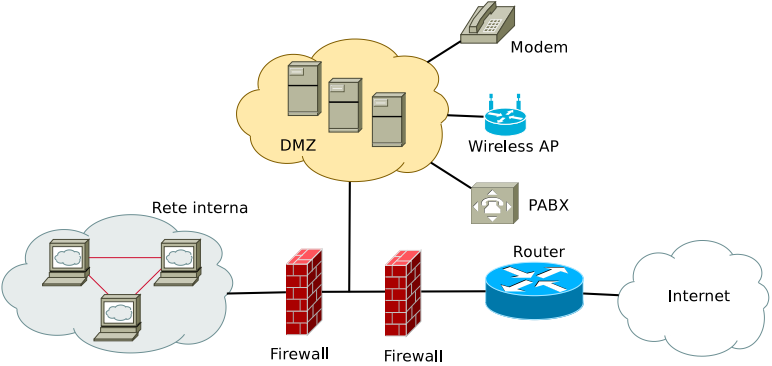
\includegraphics[scale = 0.5]{images/double-firewall}
	\caption{Configurazione a doppio firewall.}
	\label{img:double-firewall}
\end{figure}
In un'altra configurazione (Figura \ref{img:double-firewall}) possiamo immaginare di aggiungere un ulteriore firewall in modo da avere due elementi di difesa prima di arrivare alla rete corporate. Questa configurazione è più robusta, perché:
\begin{enumerate}
	\item Un attaccante dovrebbe bucare i due firewall prima di arrivare alla rete corporate (i firewall utilizzeranno software o hardware diversi, offrendo ridondanza);
	\item La DMZ è separata anche dall'interno verso l’esterno, con lo stesso principio.
	\item È più facile separare il traffico ed altri tipi di connessione verso l'esterno che possono essere considerate meno sicure si possono inserire nella DMZ.
	\item Vi è una distribuzione del carico di lavoro.
\end{enumerate}
In questo modo il firewall a cui è connessa la rete interna può controllare anche eventuali attacchi che circolano entro la rete stessa o diretti verso l'esterno. Gli svantaggi di questa tecnica sono legati in primis ai costi, ma anche alla difficile installazione e configurazione dei due firewall.

Riassumendo, possiamo dire che oggi i firewall servono poco perché gli attacchi vengono fatti direttamente sugli host terminali, dove è possibile \textquotedblleft attaccare anche senza attaccare" (i.e. buttare giù) un firewall.

\section{Netfilter/Iptables}
\textbf{Netfilter} è un framework inserito nel kernel di GNU/Linux che permette di effettuare filtraggio dei pacchetti su un firewall software. Netfilter lavora nel \textit{kernel space}, ovvero nel nucleo del sistema operativo e mette a disposizione degli \textit{hook}, ovvero dei punti di aggancio in cui i pacchetti possono essere filtrati durante il percorso all'interno del firewall. Per configurare netfilter si usa il programma \textbf{iptables}, uno strumento che permette di inserire, cancellare ed organizzare le regole di scarto, ovvero le regole secondo cui i pacchetti vengono filtrati nel kernel. Questo esempio di regola
%\shellcmd{iptables -t filter -D INPUT --dport 80 -j ACCEPT}
\shellcmd{iptables -A INPUT -p tcp -m tcp --dport 80 -j ACCEPT}
accetta i pacchetti in arrivo sulla porta 80 (protocollo TCP); \texttt{-t filter} consente di specificare la tabella da considerare (se omesso, di default viene considerata la tabella \texttt{filter}), \texttt{-A INPUT} aggiunge una regola sul traffico in ricezione (catena), \texttt{--dport 80} criterio di match della regola, \texttt{-j ACCEPT} accetta.

Le regole sono organizzate in catene e tabelle: una catena identifica il punto all'interno del percorso nel kernel in cui avviene il filtraggio, mentre una tabella associa una funzione alla regola. Un firewall è un host a tutti gli effetti, con almeno due schede di rete, ognuna delle quali possiede un indirizzo IP. I pacchetti possono arrivare su una delle schede, essere filtrati ed essere inoltrati sull'altra (forwarding); se un pacchetto ricevuto dalla prima scheda è diretto all'IP di quella scheda, il pacchetto verrà elaborato in locale, dunque non vi è forwarding. Il firewall può inoltre generare dei pacchetti, che vengono inviati all'esterno verso altri IP su una delle due schede.
\begin{figure}[htbp]
	\centering
%	\begin{tikzpicture}[node distance=2cm]
%		\node (reteA) [rect] {Rete A};
%		\node (routing) [draw, diamond, aspect=2, below of=reteA] {Routing};
%		\node (localhost1) [rect,right of=reteA, xshift=3cm] {Localhost};
%		\node (localhost2) [rect,below of=routing, xshift=-2cm] {Localhost};
%		\node (reteB) [rect,below of=routing, xshift=2cm] {Rete B};	
%		
%		\draw [arrow] (reteA) -- (routing);
%		\draw [arrow] ($(routing.south west)$) -- (localhost2);
%		\draw [arrow] ($(routing.south east)$) -- (reteB);
%		\draw [arrow] (localhost1) -- ($(routing.south east)!0.5!(reteB.north)$); 
%	\end{tikzpicture}
	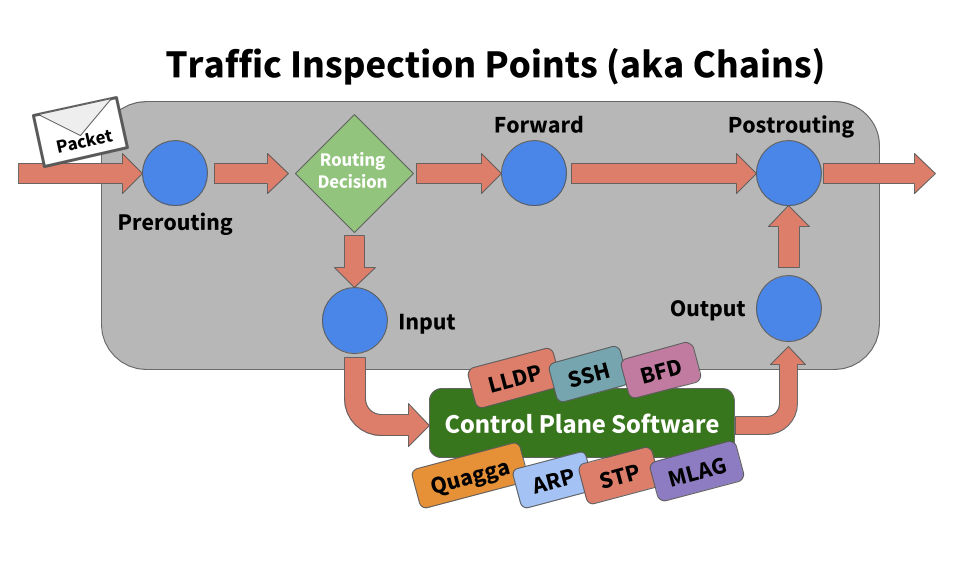
\includegraphics[scale = 0.4]{images/firewall-logic-scheme}
	\caption{Schema logico del firewall.}
	\label{img:schema-logico-firewall}
\end{figure}\\
In Figura \ref{img:schema-logico-firewall} è riportato uno schema logico del firewall. Nella parte di pre-routing entrano tutti i pacchetti in ingresso al firewall, in quella di post-routing transitano tutti i pacchetti in uscita dal firewall, nella parte di output transitano i pacchetti generati in uscita dal firewall, in quella di input i pacchetti in ingresso diretti al firewall ed infine, in quella di forward, transitano i pacchetti in ingresso al firewall ma provenienti dall'esterno. Si noti che non è possibile accorpare forward, postrouting e output sia per un motivo di duplicazione del codice, sia per il fatto che l'attaccante potrebbe provenire dall'interno.

Con il termine \textquotedblleft filtrare" ci possiamo riferire a più azioni intraprese dal firewall: scartare (Drop), lasciare passare (Accept), modificare (Mangle), lasciare passare ma riportare un messaggio nei file di log (Log), etc. Si noti inoltre che Netfilter/Iptables è \textit{stateful}, dunque vi è un modulo che ricostruisce il flusso di pacchetti correlati, ad esempio frammenti dello stesso pacchetto IP (Conntrack). Per distinguere gruppi di azioni simili, le regole vengono divise in tabelle, ovvero raggruppamenti di regole che svolgono la stessa funzione (Conntrack, Mangle, NAT, Filter). All'interno di ogni catena vengono richiamate regole appartenenti a tabelle diverse.
\begin{figure}
	\makebox[\textwidth]{
		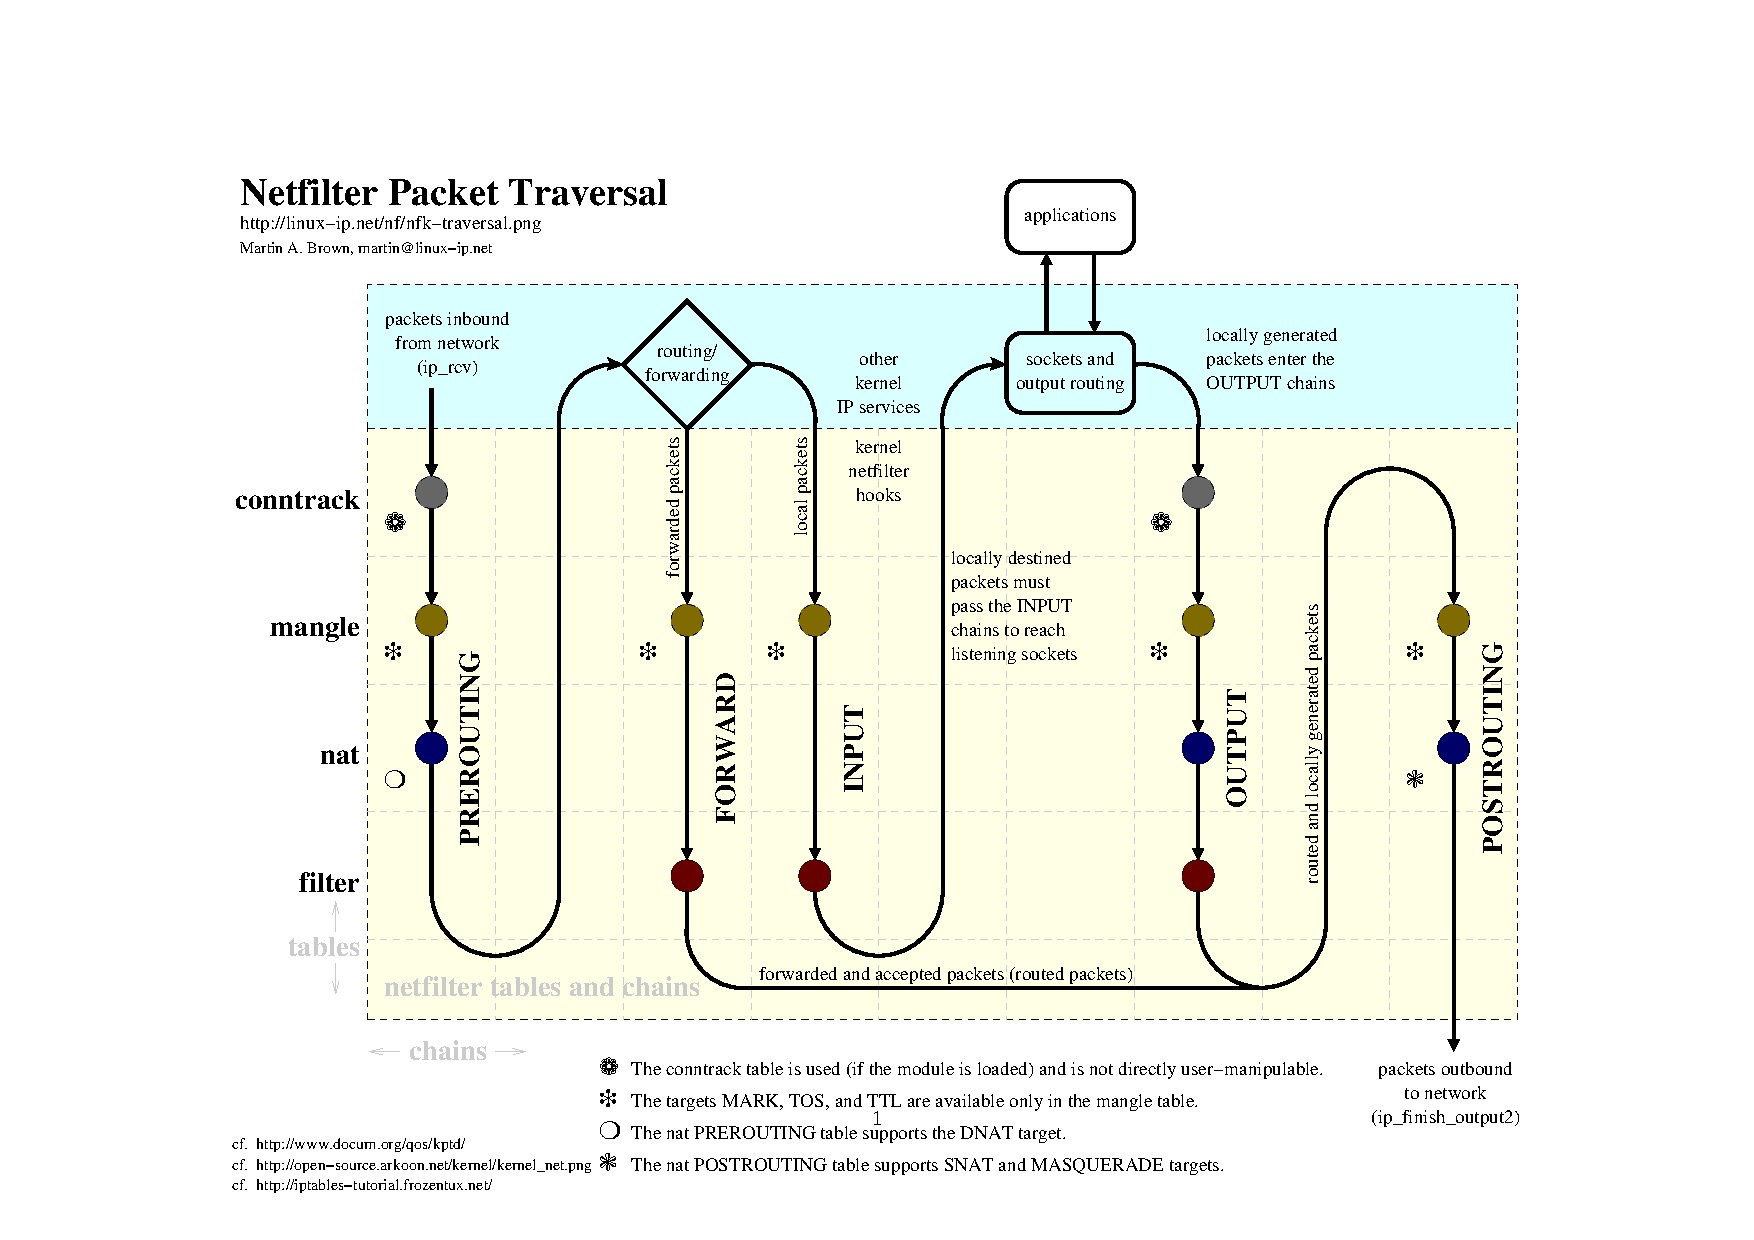
\includegraphics[width=1.3\linewidth]{images/nfk-traversal.pdf}
	}
	\caption{Schema completo di Netfilter.}
	\label{img:nfk-traversal}
\end{figure}\\
In Figura \ref{img:nfk-traversal} è rappresentato uno schema completo dei possibili percorsi che ogni singolo pacchetto può effettuare all'interno di Netfilter. Vediamo più in dettaglio le componenti lungo l'asse verticale (tables).

La tabella di \textit{NAT} (Network Address Translation) serve a modificare i campi di indirizzo IP all'interno degli header dei pacchetti. Può avere due funzionalità: DNAT e SNAT. Nel primo (Destination NAT) viene cambiato l'indirizzo IP destinazione; questa operazione viene utilizzata dai firewall di frontiera per distribuire il carico su una rete con più server. Utilizzi tipici del DNAT sono: port forwarding, in cui connessioni verso una data porta TCP o UDP dell'indirizzo esterno vengono redirette verso un particolare host della rete interna; distribuzione del carico; proxy trasparenti (e.g. Squid). Esempio:
\shellcmd{iptables -t nat -A PREROUTING -d 150.217.5.123 -j DNAT --to-destination 192.168.1.12}
Nel secondo (Source NAT) viene cambiato l'indirizzo IP sorgente; questa conversione viene utilizzata dai firewall per mascherare una rete privata, composta da indirizzi \textit{non routable}, dietro ad un indirizzo IP pubblico. L'SNAT lavora attraverso la catena di post-routing e la tabella NAT. Esempio:
\shellcmd{iptables -t nat -A POSTROUTING -s 192.168.1.12 -j SNAT --to-source 150.217.5.123}

La tabella di \textit{Filter} serve ad operare il vero filtraggio dei pacchetti, dunque decide quali far passare e quali respingere. All'interno vi è quindi una lista di regole che il firewall deve applicare a ciascun pacchetto. Al verificarsi o meno di una regola le decisioni possibili sono:
\begin{enumerate}
	\item \textit{Drop}. Il pacchetto viene scartato senza dare risposta al mittente.
	\item \textit{Reject}. Il pacchetto viene scartato inviando a destinazione una risposta di reset.
	\item \textit{Accept}. Il pacchetto continua il suo percorso all'interno del kernel.
	\item \textit{Log}. Il pacchetto genera un log (su schermo, file, etc.).
\end{enumerate}
Viene eseguito in tre punti: FORWARD, INPUT e OUTPUT.

Il modulo di \textit{Mangle} serve a cambiare la marchiatura dei pacchetti, da cui dipenderà il loro trattamento o la loro priorità. Viene eseguito per ogni pacchetto. È strettamente legato al concetto di Quality of Service.

Il modulo di \textit{Conntrack} svolge alcune funzioni fondamentali nell'azione di filtraggio, ma che vanno utilizzate con attenzione per evitare di saturare le risorse della macchina. Lo scopo è quello di mettere in relazione pacchetti diversi, secondo il funzionamento di una macchina a stati, per individuare: frammenti che costituiscono lo stesso pacchetto IP, pacchetti che fanno parte della stessa connessione, pacchetti che fanno parte di connessioni distinte ma relazionate tra loro (ad esempio connessioni FTP). Effettua quindi il \textit{tracking delle connessioni}. Vediamo un classico esempio di ruolo che può essere svolto da un Conntrack. Generalmente, in un firewall che protegge una rete privata, non si vogliono permettere connessioni dall'esterno verso le \textit{porte alte} (i.e. $>1024$)\footnote{Il numero 1024 (10 bit) è stato ideato in un primo momento principalmente per ragioni storiche, quando Internet era ancora solamente un progetto di ricerca. Dopo il successo di Internet ed il conseguente sviluppo, questo numero si è rivelato piccolo, perché è aumentato il numero di protocolli per la comunicazione ed ognuno necessita di almeno una porta; attualmente i numeri di porta sono rappresentati su 16 bit (da 0 a 65535). I servizi su porte inferiori a 1024 sono ben noti e sono quelli più controllati in fase di configurazione del firewall, mentre quelli su porte superiori a volte vengono tralasciati (ad esempio, vorremmo non avere richieste ad un server con porta di destinazione $>1024$ -- la porta sorgente invece può essere una qualsiasi). Per utilizzare ed aprire le porte basse è necessario essere amministratori della rete.}.
\begin{figure}[htbp]
	\centering
	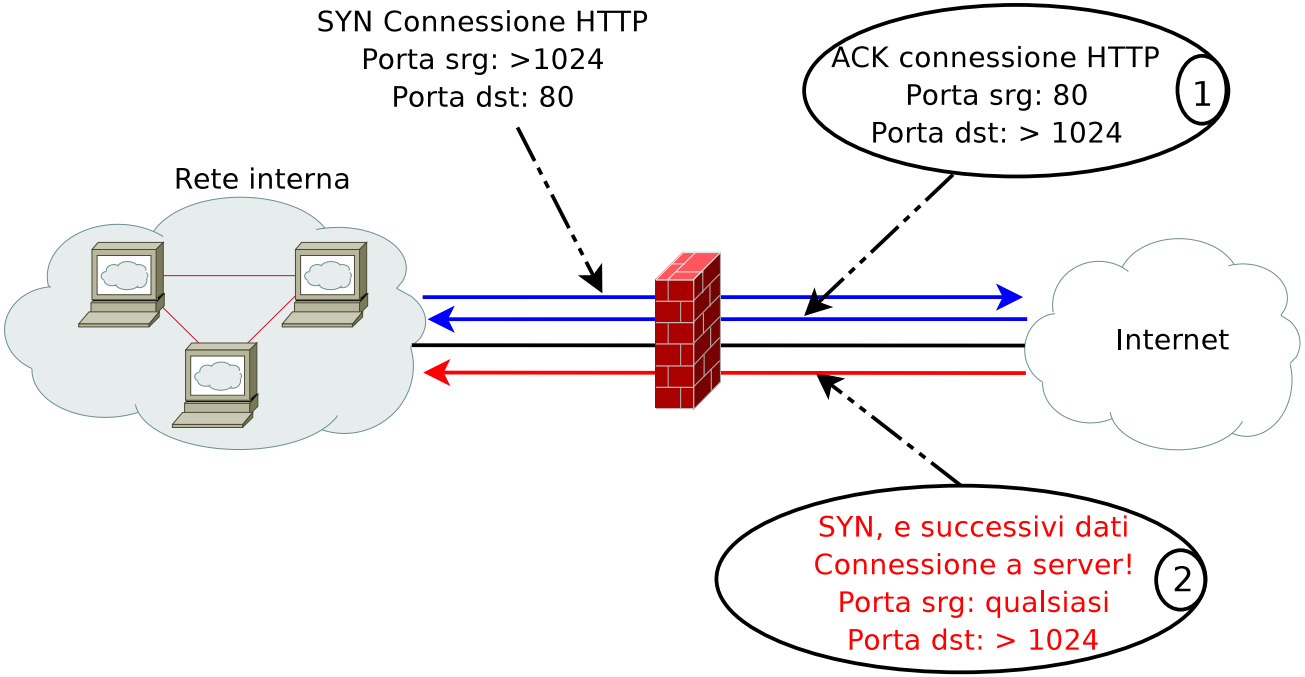
\includegraphics[scale = 0.3]{images/conntrack-example}
	\caption{Esempio di tentativo di connessione ad un host della rete interna con porta di destinazione superiore di 1024.}
	\label{img:conntrack-example}
\end{figure}\\
Nell'esempio riportato in Figura \ref{img:conntrack-example} siamo in uno scenario in cui viene effettuata una richiesta di connessione su una porta maggiore di 1024 ad un host della rete interna. Come poter distinguere i pacchetti 1 e 2 attraverso Conntrack? L'idea di verificare in base al tipo di pacchetto (SYN) non è conveniente, poiché il problema non verrebbe risolto per altri protocolli (e.g. UDP). Si nota però che esiste una differenza fondamentale: il pacchetto 1 viene ricevuto dopo aver inviato un pacchetto in uscita, mentre il pacchetto 2 invece inizia la connessione. Il modulo conntrack tiene traccia di queste associazioni. Ogni pacchetto di qualsiasi tipo (UDP, TCP) viene inserito in una\textit{connessione} che può trovarsi in quattro stati:
\begin{itemize}
	\item \textbf{NEW}. Il kernel ha visto passare pacchetti in una sola direzione.
	\item \textbf{ESTABLISHED}. Il kernel ha visto passare traffico in entrambe le direzioni.
	\item \textbf{INVALID}. Nessuna delle precedenti, si è verificato un errore.
	\item \textbf{RELATED}. Per usi specifici, il pacchetto appartiene ad una connessione in qualche modo relazionata ad una che è già ESTABLISHED.
\end{itemize}
\begin{figure}[htbp]
	\centering
	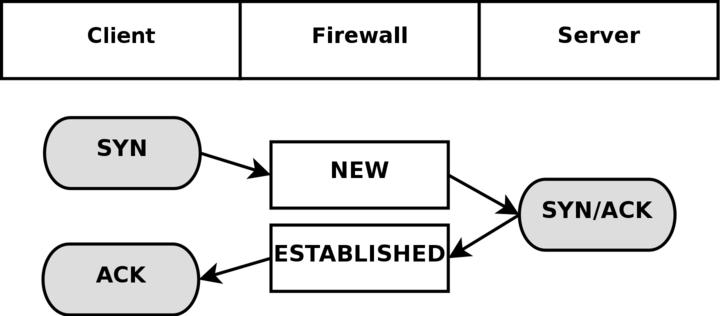
\includegraphics[scale = 0.35]{images/conntrack-state-machine}
	\caption{Macchina a stati di Conntrack per connessioni TCP.}
	\label{img:conntrack-state-machine}
\end{figure}
Una connessione TCP è sempre iniziata con il three-way handshake, che stabilisce e negozia la connessione effettiva su cui verranno inviati i dati. L'intera sessione è iniziata con un pacchetto SYN, poi un pacchetto SYN/ACK e, infine, un pacchetto ACK per riconoscere lo stabilimento dell'intera sessione.\\
In Figura \ref{img:conntrack-state-machine} è rappresentata la macchina a stati di Conntrack. Il client invia un pacchetto (SYN), il firewall lo riconosce e considera la connessione NEW. Una volta che vede il pacchetto di ritorno (SYN/ACK), il firewall considera la connessione ESTABLISHED. Nella pratica:
\shellcmd{iptabels -A INPUT -j ACCEPT -p tcp -m state --state ESTABLISHED}
\shellcmd{iptabels -A OUTPUT -j ACCEPT -p tcp -m state --state NEW, ESTABLISHED}
\shellcmd{iptables -P INPUT DROP}

\section{Bilanciamento del carico e tolleranza ai guasti}
Il firewall è normalmente un punto in ingresso e di uscita dalla rete e può costituire un collo di bottiglia. In reti che sono soggette ad alti volumi di traffico è importante condividere il carico tra più firewall per avere prestazioni migliori e ad avere procedure di backup per la tolleranza ai guasti. Vediamo due tipi di backup (esistono anche altre configurazioni):
\begin{enumerate}
	\item \textbf{Backup cold swap}. Vi sono due firewall: uno lavora e l'altro, uguale al primo, è spento o con funzionalità minimali. Non appena si guasta il primo si accende ed entra in funzione il secondo. Uno degli aspetti negativi è il downtime dovuto al tempo di accensione del firewall, mentre uno degli aspetti positivi è che consuma poca energia.
	\item \textbf{Backup hot swap}. Vi sono due firewall: uno lavora e l'altro, uguale al primo, è sempre acceso ed entra in funzione quando il primo smette di funzionare. Gli aspetti negativi e positivi sono duali alla precedente soluzione. Contrariamente all'intuizione, in questa configurazione il firewall di backup si consuma meno: generalmente i principali guasti ad una macchina sono dovuti agli sbalzi di tensione sulla piastra madre, che si verificano soprattutto durante l'accensione e lo spegnimento.
\end{enumerate}
\begin{figure}[htbp]
	\centering
	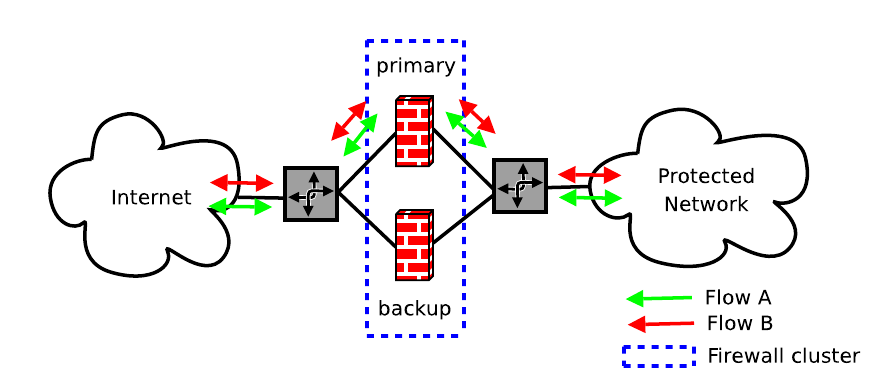
\includegraphics[scale = 0.35]{images/primary-configuration-backup}
	\caption{Primary-configuration backup.}
	\label{img:primary-configuration-backup}
\end{figure}
L'aspetto negativo di queste due soluzioni è l'elevato costo di realizzazione. Le configurazioni descritte finora sono dette \textit{primary-backup configuration} (Figura \ref{img:primary-configuration-backup}): il gateway smista il traffico ai due firewall, il primary possiede un indirizzo virtuale (VIP) che è lo stesso che vedono le applicazioni dall'esterno; il server di backup è generalmente inattivo. Si usa quindi un protocollo di \textit{heartbeat} (VRRP, HSRP, etc.) per controllare lo stato del server primario e quando questo subisce un guasto il VIP viene assegnato al server di backup. Così facendo, però, non vi è \textit{load balancing} e spreco di risorse (una macchina non fa niente); inoltre, nel momento del guasto tutte le connessioni cadono.

Un'idea migliore, che mira a distribuire il carico è la tecnica di \textit{multi-primary multi-path firewall cluster}. L'idea è identica alla precedente, viene semplicemente aggiunto un load balancer prima della coppia di firewall che distribuisce i flussi di traffico su entrambe le macchine. Così facendo vi è load balancing, ma se un solo firewall si guasta, tutte le connessioni da/verso esso si interrompono.
\begin{figure}[htbp]
	\centering
	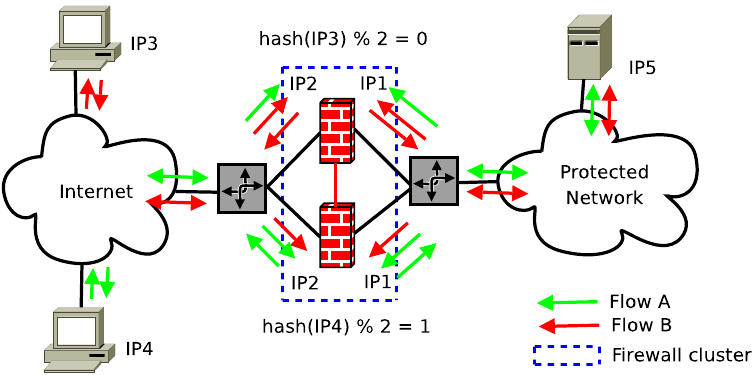
\includegraphics[scale = 0.35]{images/multi-primary-hash-based-stateful-firewall-clusters}
	\caption{Multi-primary hash-based stateful firewall-clusters.}
	\label{img:multi-primary-hash-based-stateful-firewall-clusters}
\end{figure}

Un'altra idea ancora prende spunto dalle precedenti, ma prevede l'utilizzo di entrambi i firewall: \textit{multi-primary hash-based stateful firewall-clusters} (Figura \ref{img:multi-primary-hash-based-stateful-firewall-clusters}). In questo caso non è presente un load balancer, il traffico è distribuito semplicemente attraverso il calcolo di una funzione hash. In pratica, ad ogni firewall è assegnato un ID numerico ($0,1,\dots$) ed ogni connessione in ingresso viene valutata attraverso una tupla $T = (IP_s, IP_d, Port_s, Port_d, Protocol)$. Viene quindi definita una funzione hash $h$ e, per ogni tupla $T$ in ingresso, ciascuno dei due firewall calcola $h\bmod 2$: se il risultato corrisponde al proprio ID, il firewall procede al filtraggio, altrimenti ignora la tupla. In questo modo i firewall si distribuiscono il traffico autonomamente, ma vi è comunque necessità di un heartbeat in caso di guasto.

In tutte queste situazioni, quando un firewall si guasta, si perdono le connessioni attive in quel momento. Per evitare questo inconveniente è necessario che nel momento in cui una connessione cambia stato su un firewall, questo venga replicato nell'altro (\textit{state replication}); ogni firewall, dunque, conosce sia il proprio stato sia quello dell'altro. È possibile realizzare questa idea attraverso due politiche:
\begin{itemize}
	\item \textbf{Event based}. In questo caso, ad ogni cambio di stato, questo viene inviato all'altro firewall.
	\item \textbf{Update periodici}. In questo caso viene fissato un periodo al termine del quale lo stato viene inviato all'altro firewall.
\end{itemize}
Queste due strategie hanno performance diverse in termini di affidabilità, ma anche costi computazionali differenti. Nel caso in cui i due firewall abbiano un basso volume di traffico è ragionevole aspettarsi che gli stati cambino poco nel corso del tempo, dunque sono più convenienti gli aggiornamenti event based. Se, viceversa, il volume di traffico è alto, è ragionevole aspettarsi cambi di stato frequenti, dunque gli update periodici sono più convenienti; si noti che se comunque gli aggiornamenti non sono abbastanza frequenti vi è il rischio, al momento del guasto, di avere una copia inconsistente dello stato.
\begin{figure}[htbp]
	\centering
	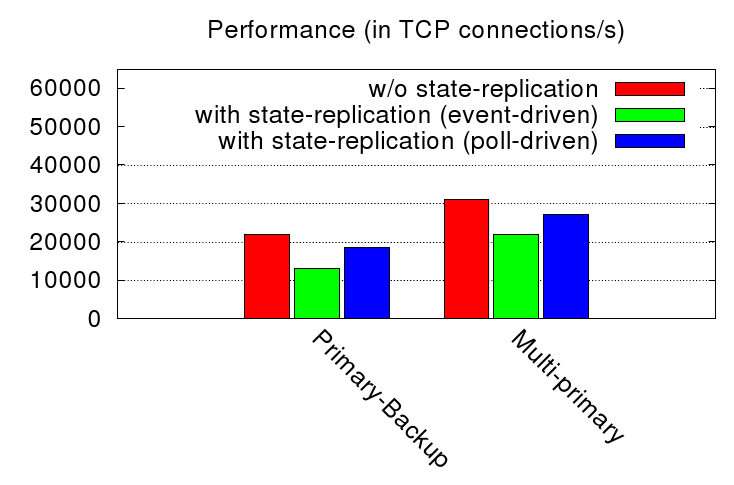
\includegraphics[scale = 0.35]{images/state-replication-performance}
	\caption{Performance con e senza state replication.}
	\label{img:state-replication-performance}
\end{figure}
A livello esemplificativo, in Figura \ref{img:state-replication-performance} sono riportate le performance, in termini di numero di connessioni TCP al secondo, con e senza state replication.

\section{L7 Filtering}
Un amministratore di rete potrebbe voler filtrare traffico di livello applicazione per vari motivi:
\begin{itemize}
	\item \textit{Log ed analisi del traffico}. Vogliamo sapere ad esempio quale è il tipo di traffico che passa attraverso la nostra rete per dimensionare efficacemente i collegamenti e gli apparati.
	\item \textit{Traffic shaping}. Vogliamo dare priorità ad alcuni flussi piuttosto che ad altri.
	\item \textit{Blocco di alcuni protocolli}. Vogliamo evitare che alcuni tipi di traffico passino sulla nostra rete.
\end{itemize}
L'idea è quella di filtrare a livello 7 dello stack protocollare ISO/OSI (\textit{L7 filtering}) quando utilizzare il numero di porta sorgente e destinazione non è sufficiente a capire il tipo di traffico che si sta analizzando. Filtrare protocolli di livello 7, tuttavia, è molto difficile: esistono meccanismi interni dei protocolli che rendono difficile collegare connessioni diverse alla stessa sessione (e.g. FTP, SIP, etc.), esistono protocolli che intenzionalmente cercano di offuscare il loro tipo, in modo da non essere distinguibili ed esistono protocolli cifrati. Ogni filtro dunque deve essere modellato sull'applicazione specifica e potrebbe avere una macchina a stati molto complessa. Implementare macchine a stati complicate per filtrare gigabit di traffico è computazionalmente molto pesante. È necessario avere macchine dedicate con potenza sufficiente.\\
Questa tecnica, oltre ad invadere la privacy dell'utente, ha bisogno di un costante aggiornamento poiché ogni volta che cambia un protocollo, è possibile che da un giorno al successivo un filtro smetta di funzionare causando perdita di performance (falsi negativi) o blocco di connessioni legittime (falsi positivi). Deve inoltre essere scritta una R7 Conntrack e questa risulta un'operazione difficile.

Un algoritmo di \textit{pattern matching} implementato in software ha gli stessi problemi di sicurezza di altri applicativi di livello 7, cosa che generalmente è più difficile per firewall di livello più basso. In pratica non viene analizzato il contenuto dei pacchetti, ma la sequenza dei dati che vengono trasmessi; in questo modo è possibile riuscire a capire il protocollo semplicemente osservando le porte (sorgente e destinazione), quanti pacchetti arrivano e da chi. Nel caso in cui un utente stia avendo del traffico non conforme, si blocca la connessione.

Alcune vulnerabilità note sono:
\begin{enumerate}
	\item \textit{Snort RPC Preprocessing Vulnerability}: \textquotedblleft Researchers at Internet Security Systems (ISS) discovered a remotely exploitable buffer overflow in the Snort stream4 preprocessor module [...] Remote attackers may exploit the buffer overflow condition to run arbitrary code on a Snort sensor".
	\item \textit{Trend Micro InterScan VirusWall Remote Overflow}: \textquotedblleft An implementation flaw in the InterScan VirusWall SMTP gateway allows a remote attacker to execute code with the privileges of the daemon."
	\item \textit{Microsoft ISA Server 2000 H.323 Filter}: \textquotedblleft Remote Buffer Overflow Vulnerability. The H.323 filter used by Microsoft ISA Server 2000 is prone to remote buffer overflow vulnerability."
	\item \textit{Cisco SIP Fixup Denial of Service (DoS)}: \textquotedblleft The Cisco PIX Firewall may reset when receiving fragmented SIP INVITE messages."
\end{enumerate}

Si definisce \textbf{net neutrality} una rete a banda larga che sia priva di restrizioni arbitrarie sui dispositivi connessi e sul modo in cui essi operano, cioè dal punto di vista della fruizione dei vari servizi e contenuti di rete da parte dell'utente finale. Quando la banda a disposizione non è sufficiente, o si aumenta la banda o si fa \textit{traffic shaping}; nel secondo caso si decide di rendere prioritari alcuni traffici rispetto ad altri. Chi offre servizi quindi diventa arbitro di quale tipo di traffico è prioritario, ovvero la rete di trasporto non è più neutrale. La perdita di neutralità viene spesso vista come un tentativo di censurare alcuni contenuti dalla rete; la net neutrality al massimo livello invece comporta una riduzione della quality of service (QoS).

Generalmente i provider vendono servizi che in teoria non possono garantire. Se tutti gli utenti di un provider utilizzassero le risorse contemporaneamente queste si saturerebbero nel giro di poco tempo. I provider contano sul fatto che l'utilizzo sia eterogeneo e diversificato nel tempo. Questo approccio utilizzato dagli ISP non va d'accordo con i protocolli P2P (file-sharing, Skype, etc.), poiché riescono a sfruttare risorse anche nei momenti in cui l'utente non fa niente. Questo, insieme ad una certa avversione nata negli ultimi anni contro il P2P, ha prodotto molta attenzione sui prodotti di \textbf{Deep-Packet-Inspection} (ovvero I7 filtering). La Deep-Packet-Inspection consiste nell'analisi della prima sequenza di pacchetti di una connessione per decidere la QoS da assegnarle.

Si noti infine che un firewall è un \textit{asset} con un protection level altissimo.